\documentclass{article}
\usepackage{tikz}
\usetikzlibrary{matrix}

\begin{document}

\begin{figure}[h]
    \centering
    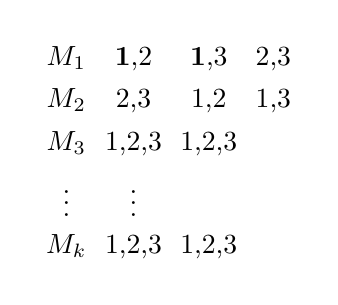
\begin{tikzpicture}
        \matrix (M) [matrix of nodes, row sep=0em, column sep=0em] {
            $M_1$ & \cellcolor{black!80}\textbf{1},2 & \cellcolor{black!80}\textbf{1},3 & 2,3 \\
            $M_2$ & 2,3 & 1,2 & 1,3 \\
            $M_3$ & \cellcolor{black!40}1,2,3 & \cellcolor{black!40}1,2,3 & \\
            $\vdots$ & $\vdots$ & & \\
            $M_k$ & \cellcolor{black!40}1,2,3 & \cellcolor{black!40}1,2,3 & \\
        };
    \end{tikzpicture}
    \qquad
    \begin{tabular}{c c c}
        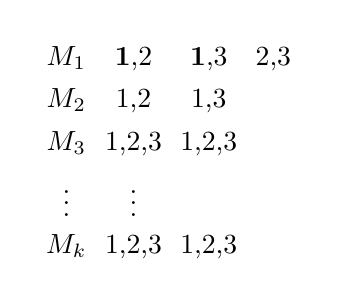
\begin{tikzpicture}
            \matrix (M) [matrix of nodes, row sep=0em, column sep=0em] {
                $M_1$ & \cellcolor{black!80}\textbf{1},2 & \cellcolor{black!80}\textbf{1},3 & 2,3 \\
                $M_2$ & 1,2 & 1,3 & \\
                $M_3$ & \cellcolor{black!40}1,2,3 & \cellcolor{black!40}1,2,3 & \\
                $\vdots$ & $\vdots$ & & \\
                $M_k$ & \cellcolor{black!40}1,2,3 & \cellcolor{black!40}1,2,3 & \\
            };
        \end{tikzpicture} &
        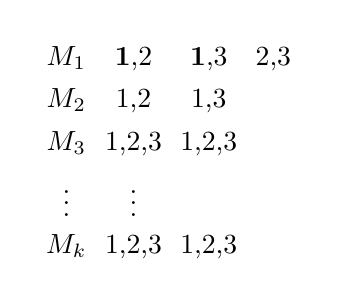
\begin{tikzpicture}
            \matrix (M) [matrix of nodes, row sep=0em, column sep=0em] {
                $M_1$ & \cellcolor{black!80}\textbf{1},2 & \cellcolor{black!80}\textbf{1},3 & 2,3 \\
                $M_2$ & 1,2 & 1,3 & \\
                $M_3$ & \cellcolor{black!40}1,2,3 & \cellcolor{black!40}1,2,3 & \\
                $\vdots$ & $\vdots$ & & \\
                $M_k$ & \cellcolor{black!40}1,2,3 & \cellcolor{black!40}1,2,3 & \\
            };
        \end{tikzpicture} &
        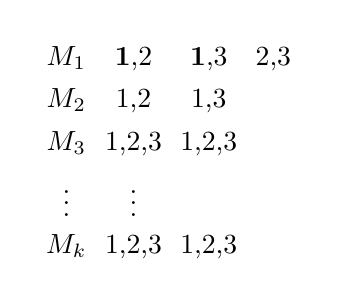
\begin{tikzpicture}
            \matrix (M) [matrix of nodes, row sep=0em, column sep=0em] {
                $M_1$ & \cellcolor{black!80}\textbf{1},2 & \cellcolor{black!80}\textbf{1},3 & 2,3 \\
                $M_2$ & 1,2 & 1,3 & \\
                $M_3$ & \cellcolor{black!40}1,2,3 & \cellcolor{black!40}1,2,3 & \\
                $\vdots$ & $\vdots$ & & \\
                $M_k$ & \cellcolor{black!40}1,2,3 & \cellcolor{black!40}1,2,3 & \\
            };
        \end{tikzpicture} \\
        $S_1$ & $S_2$ & $S_3$
    \end{tabular}
\end{figure}

\end{document}